\documentclass[border=15pt,tikz]{standalone}
\usepackage{amsmath}
\usetikzlibrary{arrows.meta, fit, positioning, backgrounds}
\usepackage[outline]{contour}
\contourlength{1.4pt}

\usepackage{helvet}
\renewcommand{\familydefault}{\sfdefault}
\usepackage{sansmath}
\sansmath

% --- COLOR DEFINITIONS (Okabe-Ito based: GraphSAGE=navy, DNN=okabe orange (solid), Output=#e74c3c) ---
\usepackage{xcolor}
\definecolor{myred}{HTML}{e74c3c}
\definecolor{myblue}{HTML}{000080}
\definecolor{mygreen}{HTML}{009E73}
\definecolor{myorange}{HTML}{E69F00}
\colorlet{mydarkred}{myred!30!black}
\colorlet{mydarkblue}{myblue!40!black}
\colorlet{mydarkgreen}{mygreen!30!black}

% --- STYLES (shared with gnn.tex / nn_qn_assignment.tex) ---
\tikzset{
  >=latex,
  base node/.style={thick, circle, minimum size=28pt, inner sep=1pt, align=center, font=\footnotesize},
  node gcn/.style={base node, draw=myblue!40!black, fill=myblue!15},
  node mlp/.style={base node, draw=myorange!40!black, fill=myorange},
  node out/.style={base node, draw=myred!40!black, fill=myred!15},
  op block/.style={thick, rounded corners=4pt, draw=myorange!40!black, fill=myorange, align=center, font=\scriptsize},
  msg edge/.style={->, thick, mydarkblue, shorten >=2pt, shorten <=2pt},
  dense edge/.style={thick, mydarkblue, opacity=0.3},
  ops arrow/.style={->, thick, line width=1.2pt, mydarkblue!80, shorten >=2pt, shorten <=2pt},
  flow arrow/.style={->, thick, line width=1.5pt, draw=black!60},
  label/.style={font=\small\bfseries, align=center},
  desc/.style={font=\scriptsize, align=center, text=black!80},
  box/.style={draw, thick, rounded corners=6pt, inner sep=14pt, fill opacity=0.05}
}

\begin{document}

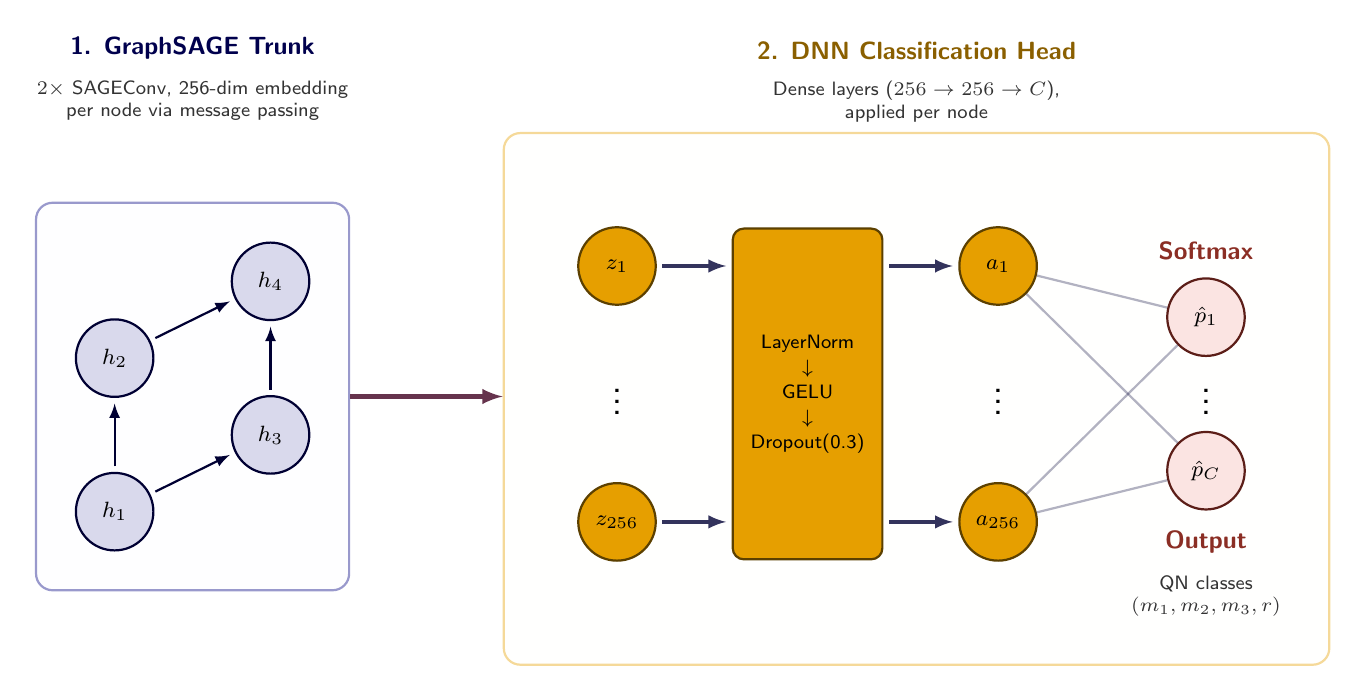
\begin{tikzpicture}[x=2.2cm, y=1.3cm, font=\sffamily]

  % =================================================================================
  % SECTION 1: GRAPHSAGE TRUNK (message passing)
  % =================================================================================

  \node[node gcn] (H1) at (2.9, 1.0)  {$h_1$};
  \node[node gcn] (H2) at (2.9, 2.5)  {$h_2$};
  \node[node gcn] (H3) at (3.8, 1.75) {$h_3$};
  \node[node gcn] (H4) at (3.8, 3.25) {$h_4$};

  % Message passing along the physical graph topology
  \draw[msg edge] (H1) -- (H2);
  \draw[msg edge] (H3) -- (H4);
  \draw[msg edge] (H1) -- (H3);
  \draw[msg edge] (H2) -- (H4);

  \begin{pgfonlayer}{background}
    \node[box, fit=(H1) (H2) (H3) (H4), fill=myblue!5, draw=myblue!40] (box-trunk) {};
  \end{pgfonlayer}

  \node[label, myblue!60!black, above=48pt of box-trunk.north] (Title1) {1. GraphSAGE Trunk};
  \node[desc, below=1pt of Title1] {$2\times$ SAGEConv, 256-dim embedding\\per node via message passing};


  % =================================================================================
  % SECTION 2: DNN CLASSIFICATION HEAD
  % =================================================================================

  % Layer 1: trunk embedding (256)
  \node[node mlp] (Z1) at (5.8, 3.4) {$z_1$};
  \node[node mlp] (Z2) at (5.8, 0.9) {$z_{256}$};
  \path (Z1) -- (Z2) node[midway, font=\Large] {$\vdots$};

  % Post-linear operation stack between the two parallel dense layers
  \node[op block, minimum width=1.9cm, minimum height=4.2cm] (ops) at (6.9, 2.15)
    {LayerNorm\\[1pt]$\downarrow$\\[1pt]GELU\\[1pt]$\downarrow$\\[1pt]Dropout(0.3)};

  % Layer 2: hidden dense layer (256), parallel to layer 1
  \node[node mlp] (A1) at (8.0, 3.4) {$a_1$};
  \node[node mlp] (A2) at (8.0, 0.9) {$a_{256}$};
  \path (A1) -- (A2) node[midway, font=\Large] {$\vdots$};

  % Layer 3: class probabilities (softmax output)
  \node[node out] (P1) at (9.2, 2.9) {$\hat p_1$};
  \node[node out] (P2) at (9.2, 1.4) {$\hat p_C$};
  \path (P1) -- (P2) node[midway, font=\Large] {$\vdots$};
  \node[label, myred!60!black] (smx) at (9.2, 3.55) {Softmax};
  \node[label, myred!60!black] (outlbl) at (9.2, 0.7) {Output};
  \node[desc, below=1pt of outlbl] (outdesc) {QN classes\\$(m_1, m_2, m_3, r)$};

  % Invisible pad: its x mirrors the labels' right overhang, its y balances the
  % Output stack below, so the circles/block sit dead-centre in the fitted box
  \coordinate (headpad) at (5.37, 4.32);

  % z -> ops block -> a
  \draw[ops arrow] (Z1) -- (ops.west |- Z1);
  \draw[ops arrow] (Z2) -- (ops.west |- Z2);
  \draw[ops arrow] (ops.east |- A1) -- (A1);
  \draw[ops arrow] (ops.east |- A2) -- (A2);

  % Fully connected dense edges (final Linear, 256 -> C)
  \draw[dense edge] (A1) -- (P1);
  \draw[dense edge] (A1) -- (P2);
  \draw[dense edge] (A2) -- (P1);
  \draw[dense edge] (A2) -- (P2);

  \begin{pgfonlayer}{background}
    \node[box, fit=(Z1) (Z2) (ops) (P1) (P2) (smx) (outlbl) (outdesc) (headpad), fill=myorange!5, draw=myorange!40] (box-head) {};
  \end{pgfonlayer}

  \node[label, myorange!60!black, at={(box-head.north |- Title1.south)}, anchor=south] (Title2) {2. DNN Classification Head};
  \node[desc, below=1pt of Title2] {Dense layers ($256 \to 256 \to C$),\\applied per node};


  % =================================================================================
  % MACRO FLOW CONNECTIONS
  % =================================================================================

  \draw[flow arrow, draw=myblue!60!orange]  (box-trunk.east) -- (box-head.west |- box-trunk.east);

\end{tikzpicture}

\end{document}
